\section{Introduction}
\label{ch:intro}

\epigraph{That men do not learn very much from the lessons of history is the most important of all the lessons that history has to teach.}{Aldous Huxley}

\subsection{History of Recommendation System}
Review the changes in the way we look for information so far since the birth of the Internet. In the earliest days, information was scarce. The scattered information led to low efficiency of searching. The main method of information transmission was that people looking for information. Later, the information has gradually been enriched. Some people or companies have gathered kinds of information on some websites, and people can search through the category navigation.
\par With the increasing amount of information, artificially added categories can no longer cover all information, so another type of information acquisition way - search, is born. Typical companies are Google and Baidu.
\par With the development of communication technology and data science, the relationship between people and information has evolved from one-way people looking for information to the current two-way relationship. People find what they need in massive amounts of information, and at the same time, massive amounts of information are also find ways to matching with the audience.
\par Balabanovic designed an adaptive agent for automated web browsing\cite{balabanovic1996adaptive}, in which we can see the prototype of the original recommendation system. Such traditional recommendation systems are unsatisfactory because most of the recommendation systems we use today only make recommendations. Users do not understand the reason and meaning of recommendations. In many cases, if the recommendation algorithm is not accurate or is completely wrong, the results of the recommendation will be strange and deepen the users' doubts and distrust. Recommendations are generated by the entire black-box operations. Users cannot choose but passively accept recommendations and cannot improve the effect of recommendation through interaction.
\par Yongfeng et al. introduced " Explainable Recommendation " which was a new survey and perspectives for recommendation system\cite{zhang2018explainable}. However, much of the research up to now has been descriptive in the generation of explanation. What we can do with explanations and what feedback users can give to the system about the explanation. Based on feedback on explanations, what optimizations can the recommend system make for that and how can it make such optimizations. Little research has been done on these issues.
\par In this paper, we compare the different ways in 5 recommendation styles, provide an overview of the relationship among recommend system, recommendation explanation, and explanation adaptation. We explore the ways in which design an adaptation style for the recommendation explanation module and feedback scoring module. And we propose a new methodology for the "adaptation rule" or "adaptation algorithm" of recommendation explanation.
\par From this evolutionary process, we can see that the emergence of recommendation systems has two important prerequisites, one is information overload, and the other is ambiguous requirements. With the rapid development of today's technology and the increasing amount of data, people feel more and more helpless in the face of massive data. In order to solve the problem of information overload, the computer scientists have proposed a recommendation system, which corresponds to a search engine and can also be referred to as a recommendation engine.
\par Search engines require people to have a clear purpose. They can turn people ?s search for information into precise keywords, then give them to the search engine and finally return them to a series of lists. Users can give feedback on these results. But it will have the problem of the Matthew effect\cite{merton1968matthew}, which will cause the more popular things to become more popular as the search process iterates, making those less popular things sink to the sea.
\par The recommendation engine is more suitable for people who have no clear purpose, or that their purpose is ambiguous. Generally speaking, the user does not even know what he wants. The user's historical behavior or the user's interest preferences or the user's demographic characteristics are transmitted to the recommendation system, and then the recommendation system uses some algorithm to generate a list of items that the user may be interested in. The user is passive to search engines. People only focus on high-exposure items and ignore low-exposure items, which is called the long-tail theory\cite{anderson2004long}, can be used to explain the correctness and rationality of the recommendation system well. Experiments have shown that the low-exposure items in the long tail position generate no less than profit from selling only high-visibility items. The recommendation system can provide opportunities for all items to be recommended, for discovering the potential profits of long-tail projects.
\par When a user's needs are clear, he tends to use search. When the requirements of the user are not clear, some behaviors and preferences data based on the user's history can be used to generate a pre-recommendation, to make the user stay in the system. Some new demands may arise during the user's browsing of information.
\par From the above sections, we can see that the recommendation system is a multi-win-win thing:
\par For users, they can discover what they are interested in and improve the user experience;
\par For items, it is possible to discover the utilization efficiency of long-tail items and revitalize the overall resources;
For the platform, it is able to capture user value and business value.

\subsection{Interaction Between People and Internet}
We can divide the scenarios where people interact with the Internet into three situations as shown in figure \ref{figure:1-1}.

\begin{figure}[h]
\caption{Interaction styles between people and Internet}
\label{figure:1-1}
\centering
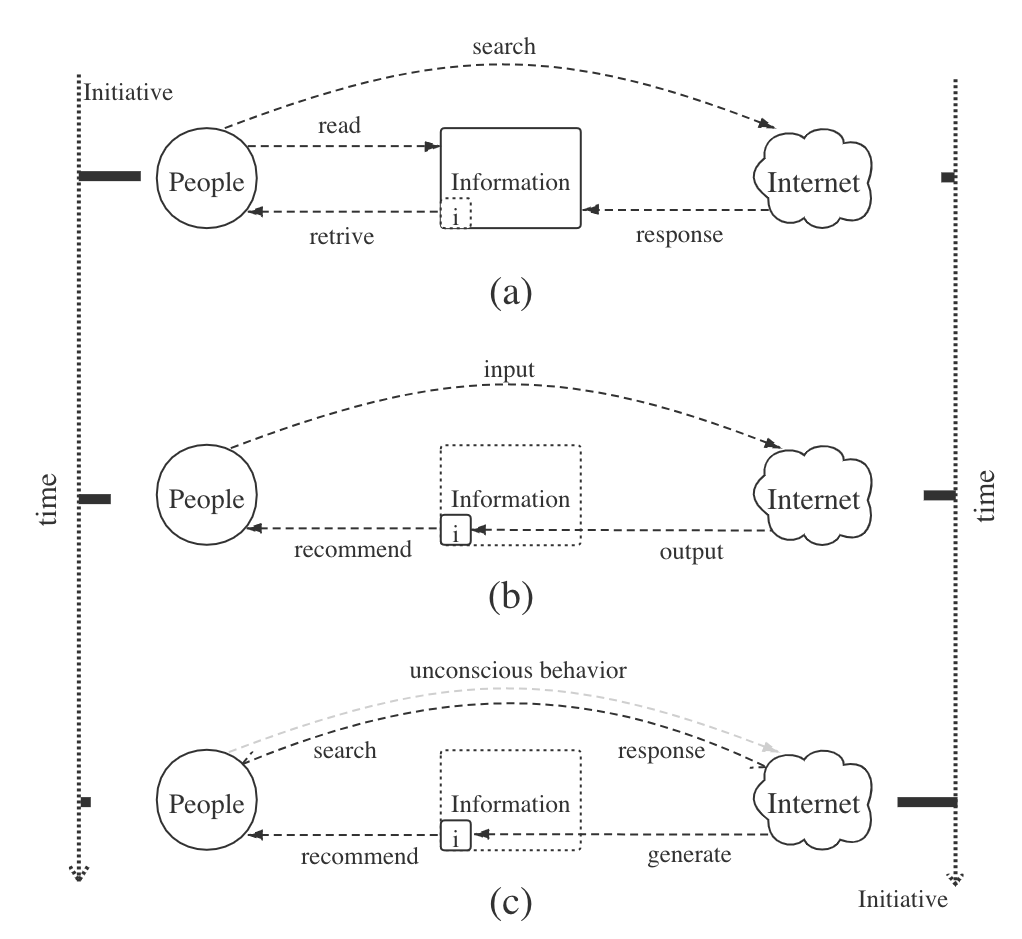
\includegraphics[width=0.8\textwidth]{people_internet_interaction}
\end{figure}

\par \textbf{(a):} People proactive use search engines to get information, and the Internet generates corresponding search results based on what users search for and returns the results according to some organizational structure. The volume of this information "I" is very large and complex. People read this information "I" and try to find the information "i" (i $\in$ I) they need and extract it.
\par \textbf{(b):} People enter some information, and the Internet outputs some recommendations through a recommendation system, and selects a small part of the information that the user needs from a huge information stream, and sends it to the user.
\par \textbf{(c):} The recommendation engine actively searches for audiences that match the content it is recommending, collects data generated by users' unconscious behaviors on the Internet, and analyzes it. In addition, it will actively generate information and recommend that to the corresponding people. For example, a customer purchased a certain product x on Amazon. After a few days, he watched the video on Youtube and found that the advertisement before the video was put by the manufacturer of product x. And the advertising content was about another product y similar to product x. This is one of the ways in which (c) interaction scenarios simply appear in our lives. In the future, human interaction approaches for the recommendation engine based on the scenario (c)  will be more natural and diverse.
\par From a vertical perspective, over time and the development of computer technology. Human initiative is decreasing, and correspondingly, Internet initiative is increasing. This may be the trend of future recommendation system development.
\par Internet giants such as Google and Baidu, which relied on the advantages of search engine technology in the early days, quickly grew into giant companies in the Internet industry. With the development of Internet technology and computing science today, the speed of information generation and transmission is getting faster and faster, and the volume is getting larger and larger. The recommendation system plays a very important and irreplaceable role in the interaction between people and the Internet, as described in (b). But on the other hand, we can see in (c) that recommendation engines have great development potential to achieve the same magnitude as search engines. In this paper, we will do some valuable research and exploration in aspects such as explanation and adaptation for recommend system.

\subsection{Our Contributions}
In this paper, we compare the different ways in 5 recommendation styles, provide an overview of the relationship among recommend system, recommendation explanation, and explanation adaptation. We explore the ways in which design an adaptation style for the recommendation explanation module and feedback scoring module. And we propose a new methodology for the "adaptation rule" or "adaptation algorithm" of recommendation explanation.

\cleardoublepage